\chapter{Resultados e Discussão}\label{cap:resultados}

\section{Sequenciamento e controle de qualidade das leituras}
Após o sequenciamento das amostras, foram obtidas 7.8 milhões de leituras de tamanho médio de 
223 pares de base para a amostra ACT016 e 7.4 milhões de leituras com tamanho médio de 222 pares de base
para a amostra ACT094. Após a filtrar as leituras utilizando a ferramenta Trimmomatic, retivemos
6.2 milhões de leituras com tamanho médio 113 pares de base \(perda 21,5\%\) para ACT016 e 6.1 milhões
de leituras com tamanho médio 145 pares de base\(perda de 18,5\%\).

Baseando-se num tamanho de genoma variável de 3 a 10 milhões de bases para \textit{Rhodococcus}, podemos
determinar a cobertura real estimada pela fórmula $C= (L\cdot N)/G $ sendo $C$ a cobertura, $L$ o comprimento
médio das reads e $G$ o tamanho do genoma. A partir disso, obtivemos que a cobertura para a amostra ACT016 Após
filtrar as leituras está entre $70$ e $233,53$ vezes. 
Para a amostra ACT094, consideramos o tamanho do genoma de referência de \textit{Brevibacillus Brevis}$($NZ\_LR134338$)$ 
de 6.2 milhões de bases e estimamos a cobertura em aproximadamente $142,66$ vezes.

As qualidades médias das sequências pode ser observada a partir dos gráficos a seguir gerados pela ferramenta FASTQC:

\begin{figure}[H]
	\caption{Gráficos representando a qualidade média das leituras da amostra ACT016 na escala PHRED}
	\label{fig:fastqc_antes}
	\centering
	\begin{minipage}{.45\linewidth}
		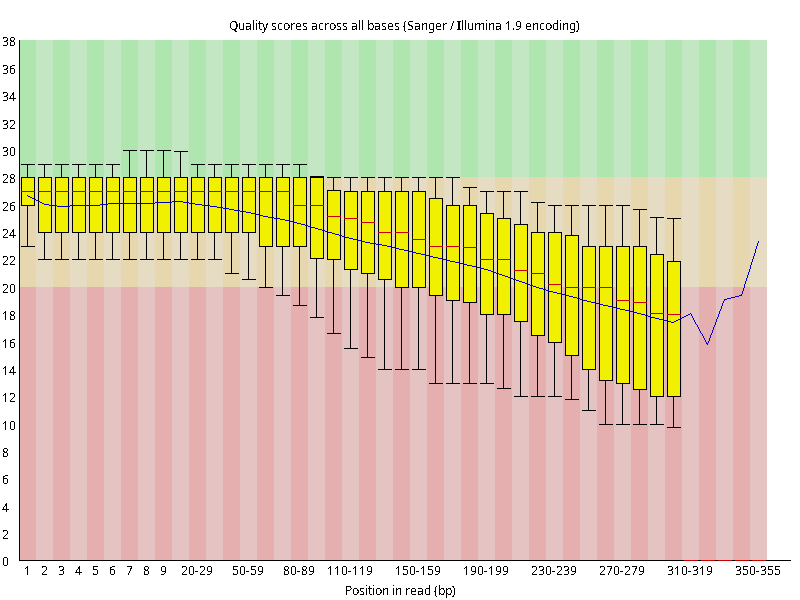
\includegraphics[height=.45\linewidth]{imagens/read\_qc/002.png}
	  \end{minipage}
	  \hspace{.01\linewidth}
	  \begin{minipage}{.45\linewidth}
		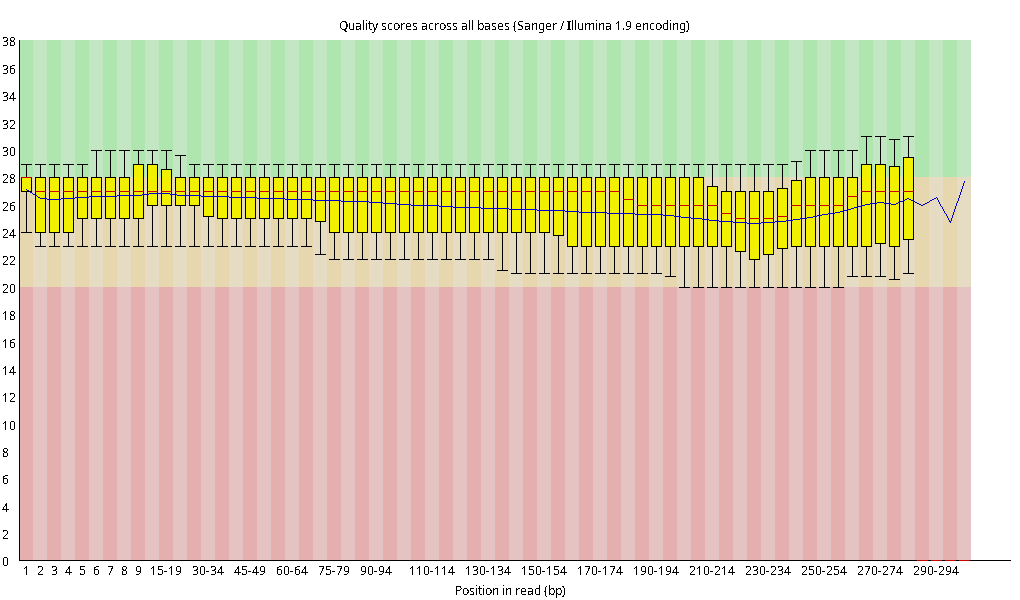
\includegraphics[height=.45\linewidth]{imagens/read\_qc/002trimmed.png}
	  \end{minipage}
	  \vspace{\floatsep}
    \begin{small}\textbf{Fonte: O Autor (2022)}\end{small}
\end{figure}
\vspace{\floatsep}
\begin{figure}[H]
	\caption{Gráficos representando a qualidade média das leituras da amostra ACT094 na escala PHRED}
	\label{fig:fastqc_antes}
	\centering
	\begin{minipage}{.45\linewidth}
		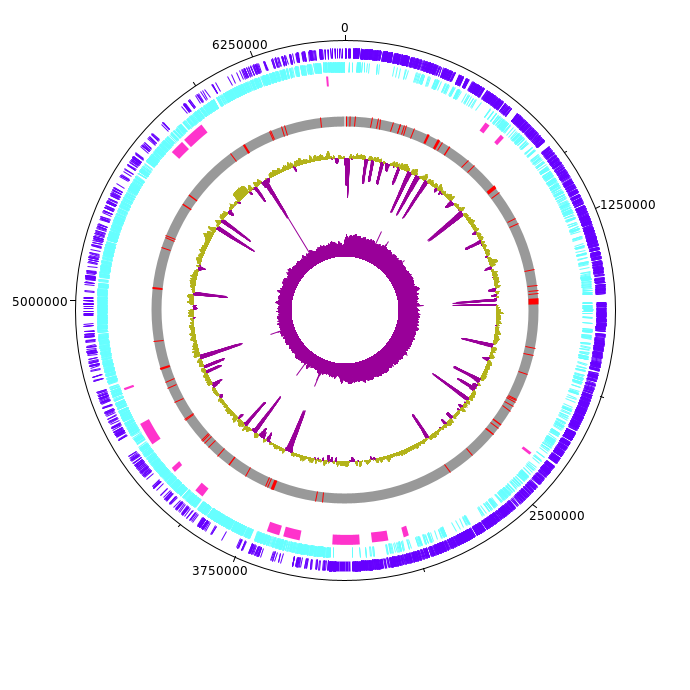
\includegraphics[height=.75\linewidth]{imagens/read\_qc/004.png}
	  \end{minipage}
	  \hspace{.01\linewidth}
	  \begin{minipage}{.45\linewidth}
		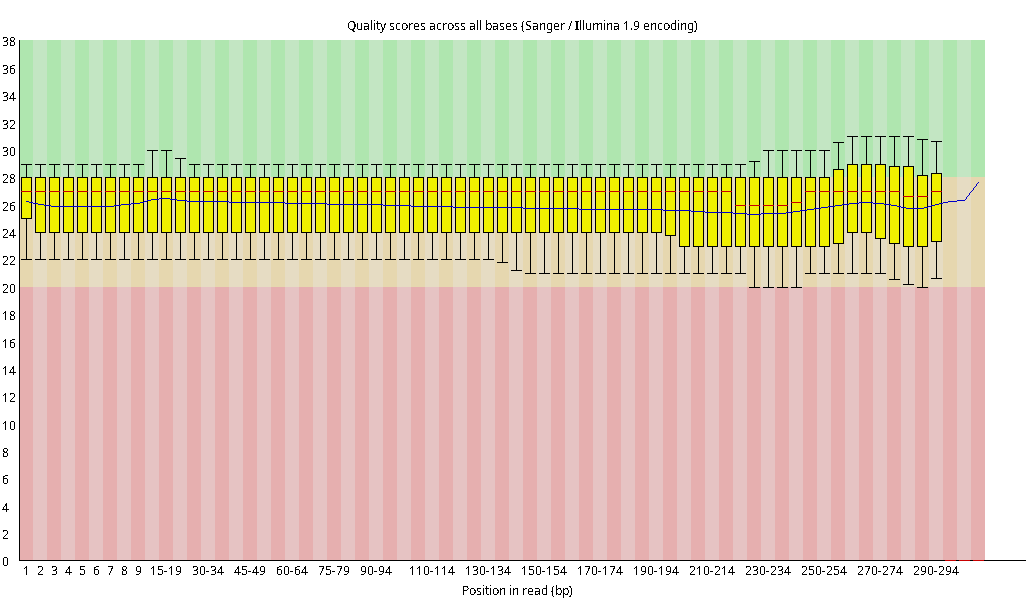
\includegraphics[height=.75\linewidth]{imagens/read\_qc/004trimmed.png}
	  \end{minipage}
	  \vspace{\floatsep}
    \begin{small}\textbf{Fonte: O Autor (2022)}\end{small}
\end{figure}
\vspace{\floatsep}

A partir desses gráficos podemos observar a perda de qualidade no final das leituras, um tipo de limitação
técnica comum ao utilizar sequenciadores da plataforma \textit{Illumina}, porém o término em baixa qualidade
pode ser removido após a filtração, tendo uma qualidade média ao longo da sequência próximo de PHRED 26 e
removendo sequências abaixo de PHRED 20 $($ que representa probabilidade de erro maior que 1 em 100$)$.


\section{Montagem das \textit{contigs}}

\subsection{016}
\begin{figure}[H]
	\caption{Report do software QUAST para as montagens da amostra 016}
	\label{fig:quast_16}
	\centering
		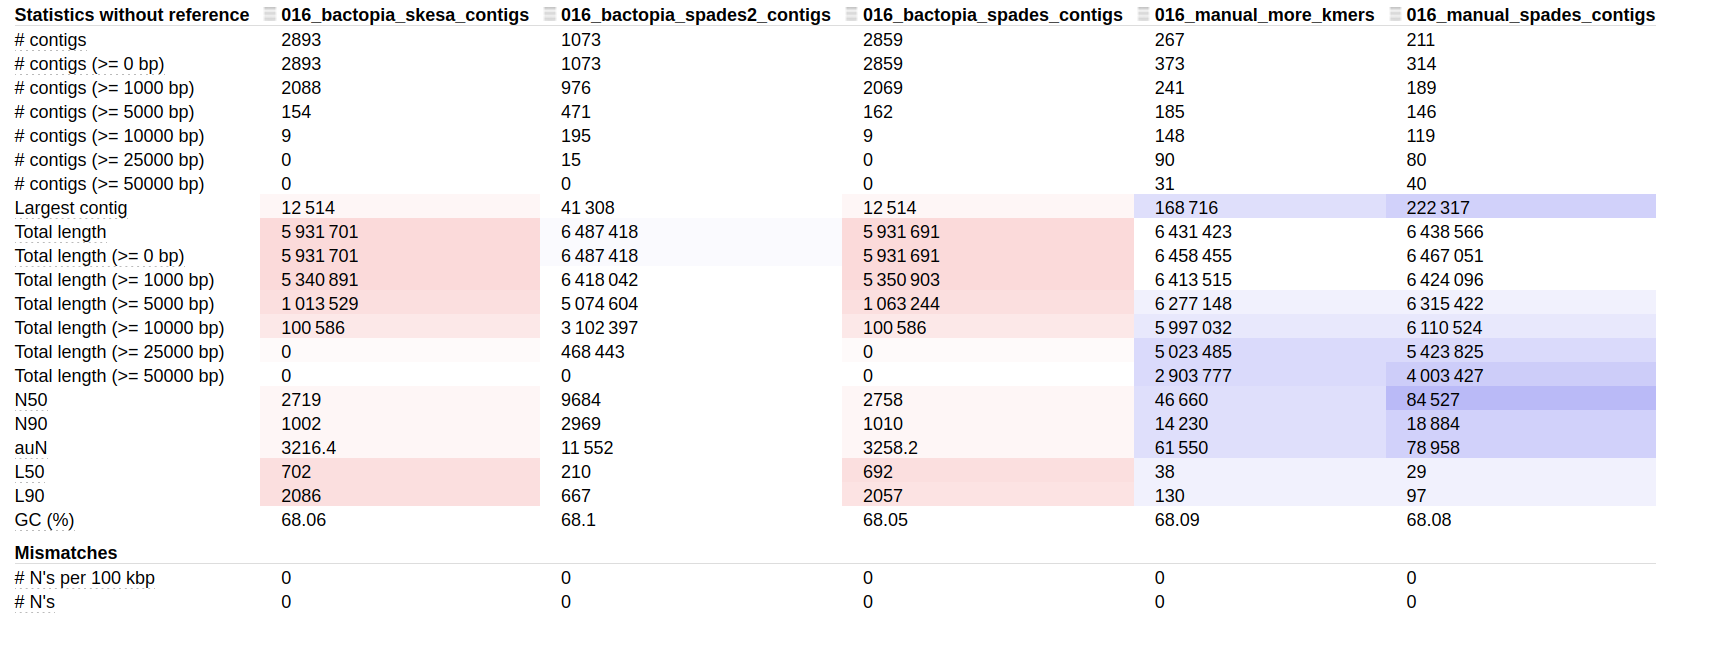
\includegraphics[width=0.45\linewidth]{imagens/assembly\_qc/016assembly.png}
		\vspace{\floatsep}
    \begin{small}\textbf{Fonte: O Autor (2022)}\end{small}
\end{figure}
\vspace{\floatsep}

A melhor montagem para a amostra ACT016 é a montagem \textit{manual\_spades} que foi feita utilizando
o montador spades junto com a correção do software shovill. Essa montagem foi escolhida por ter o maior
valor de L50 $($menor quantidade de contigs para atingir 50 \% do número de pares de base$)$ e maior 
\textit{contig} em tamanho absoluto $($222 mil pares de base$)$. O conteúdo GC de 60 \% dessa montagem está de acordo
com o descrito por \citeonline{yadav2018} para Actinomicetos.

\subsection{094}

\begin{figure}[H]
	\caption{Report do software QUAST para as montagens da amostra 094}
	\label{fig:quast_16}
	\centering
		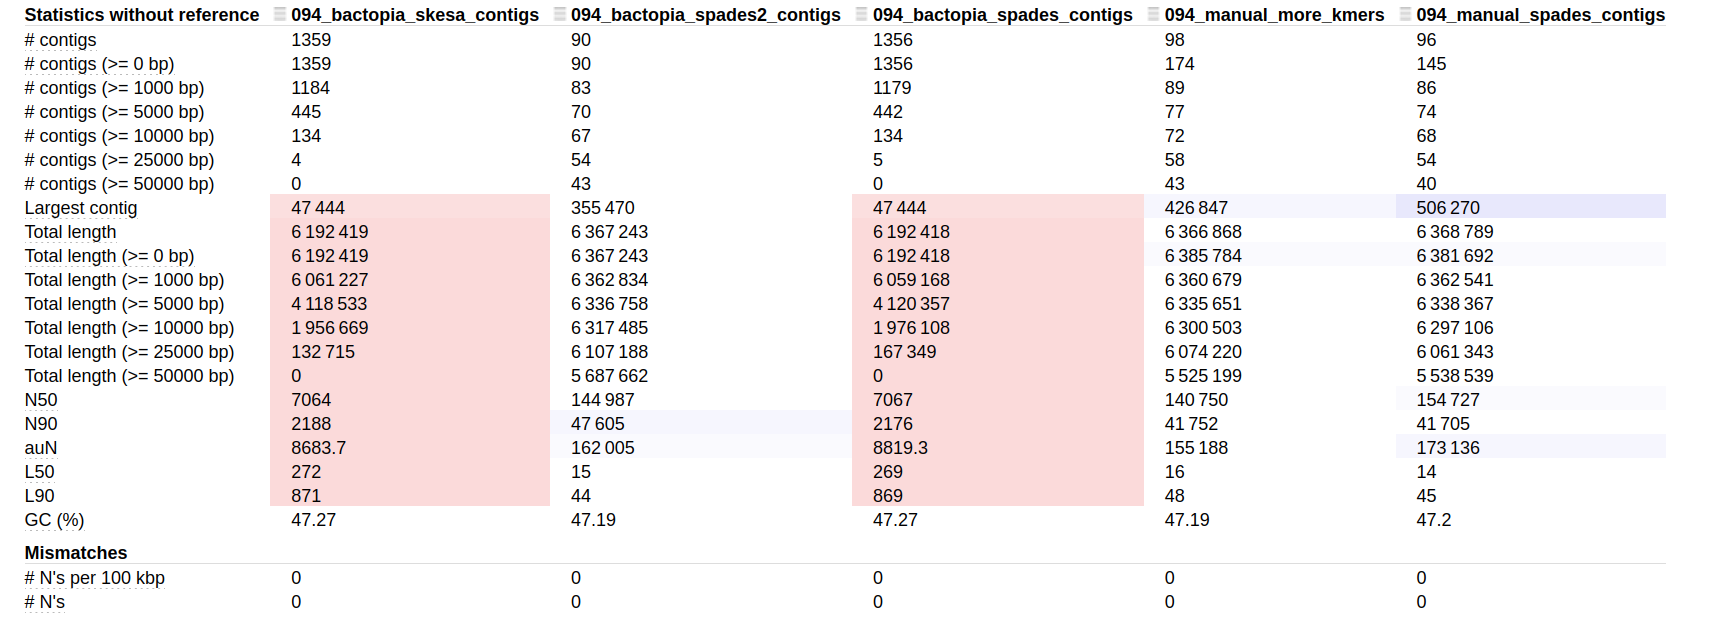
\includegraphics[width=0.45\linewidth]{imagens/assembly\_qc/094assembly.png}
		\vspace{\floatsep}
    \begin{small}\textbf{Fonte: O Autor (2022)}\end{small}
\end{figure}
\vspace{\floatsep}

De maneira similar, a melhor montagem para a amostra 094 também é a montagem \textit{manual\_spades}.
possuindo um valor similar a montagem \textit{more\_kmers} porém se diferenciando por possuir a maior \textit{contig}
com aproximadamente 80 mil pares de base a mais, um fator muito relevante para a posterior montagem do genoma completo.
O conteúdo GC também está de acordo com valores comumente encontrados em \textit{Brevibacillus brevis} \cite{nakamura1991bacillus}.

\section{Predição de espécies e montagem de genoma}

Os melhores conjuntos de \textit{contigs} montadas foram submetidas ao software KRAKEN2 para predição de espécie,
para a amostra 016 a espécie predita foram \textit{Rhodococcus} com $71,66$ \% de \textit{contigs} identificadas, mas importunamente
$18,45$ \% das \textit{contigs} não foram identificadas, determinando que a amostra 016 foi predita como \textit{Rhodococcus}
não identificado. A partir desse resultado o genoma de referência sugerido para a montagem foi o de código
de acesso NZ\_CP054690 da cepa \textit{Rhodococcus sp. W8901}. 

Para a amostra 094, $85.52$ \% das \textit{contigs} foram preditas como \textit{Brevibacillus brevis}
concordando com os resultados previamente obtidos a partir de sequenciamento de sanger. O genoma NZ\_CP030117
da cepa \textit{DZQ7} referência para montagem de genomas dessa espécie.

As montagens utilizando genomas de referência escolhidos, foram avaliadas quanto a presença de genes 
ortólogos. Na amostra 016 foram encontrados 120 BUSCOs completos e únicos, 2 genes completos e duplicados e 2 genes fragmentados,
 o valor de genes completos únicos de 98\% foi considerada satisfatória para a montagem e de pureza suficiente para
a anotação do genoma. Já na amostra 094, 121 BUSCOs completos e únicos foram encontrados, 1 gene completo e duplicado, 1 busco fragmentado
e 1 busco faltando, com o percentual de $98,4$ \% também foi considerada suficiente para prosseguimento da anotação.

o software PROKKA foi capaz de predizer 5738 CDSs para a amostra 016 e 6082 CDS para a amostra 094, contendo genes
de diversas funções celulares. 